\section{Lustre Lite}

In this section, we describe how Lustre Lite connects and fits into
Linux VFS, which is necessary for  supporting VFS semantics and the POSIX
interface. To summarize, Lustre Lite provides the following functions through
a method table:

\begin{itemize}

  \item Lustre specific file operations, through
  \url{ll_file_operations}.

  \item Lustre specific dentry operations, through \url{ll_d_ops} and
  its cache.

  \item Lustre specific directory operations, through
  \url{ll_dir_operations}.

  \item Lustre specific inode operations, through
  \url{ll_dir_inode_operations} and \url{ll_file_inode_operations}.

  \item Lustre specific file mapping operations, through
  \url{ll_file_vm_ops}.

  \item And many others, such as Lustre super block operations, address
  spaces, etc.

\end{itemize}

\begin{figure}[hbt]
\centering
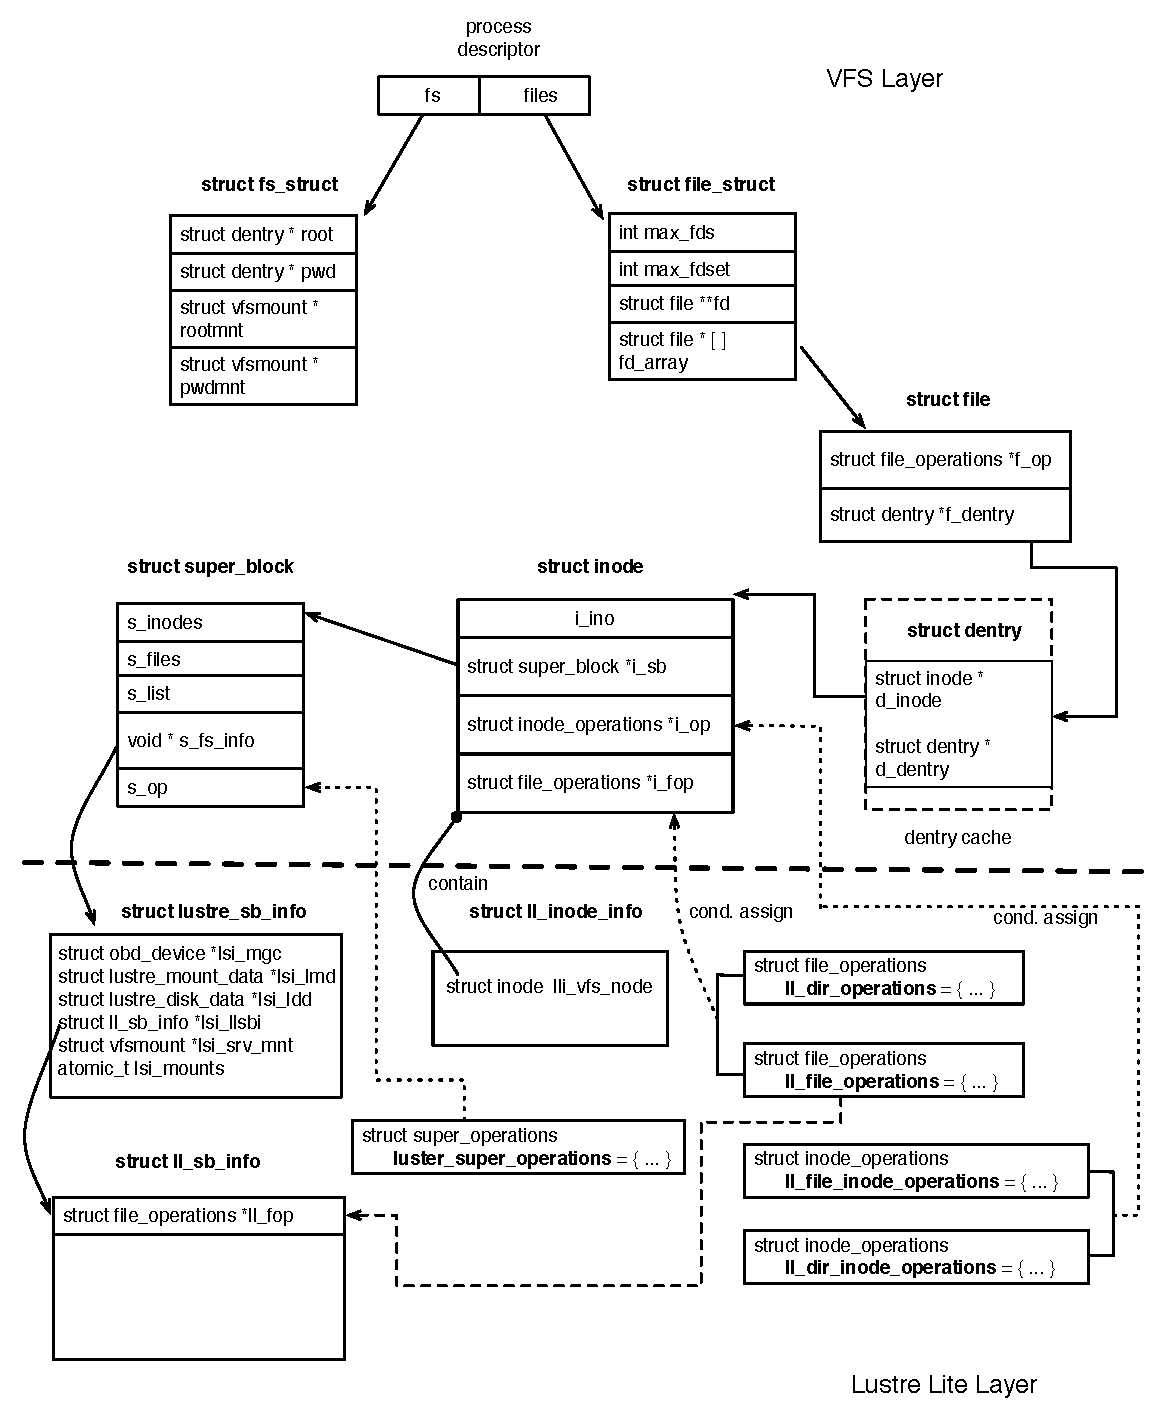
\includegraphics[width=5in]{img/lustre_vfs}
\caption{Hooking up Lustre with Linux VFS.}
\label{fig:vfs}
\end{figure}

\subsection{VFS Connection}
\label{sec:vfsreg}

Figure \ref{fig:vfs} presents an overall picture of how various data structures
are connected. Some highlights are explained below.

A process maintains a list of associated open files. Each open file has an
in-memory representation known as the \url{file} object. It stores the
information necessary to interact between an open file and process.  To the
userland, this is presented by a file handle, \url{fd}. This data structure
contains a field, \url{f_op}, that acts like a switchboard or pointer to a
method table that provides functions specific to each filesystem. So a file
read using system call \url{sys_read()} becomes: 

\begin{Verbatim} 
file->f_op->read(...);
\end{Verbatim}

\subsubsection{Dentry Object}

Another important field defined in the \url{file} structure is \url{f_dentry},
which points to a dentry object (\url{struct dentry}) stored in a dentry
cache, also known as the \textit{dcache}. Essentially, VFS will create a
dentry object  the first time a file or directory is about to be accessed. If
this is a non-existent file/directory, then a negative dentry will be
created.  As an example, take the following pathname:
\url{/home/bob/research08}; it is composed of four path components:
\url{/}, \url{home}, \url{bob}, and \url{research08}.  Correspondingly, the
path lookup will create four \url{dentry} objects for each component.  Each
dentry object associates \textit{the} respective component with its inode
through field \url{d_inode}.

The inode object stores information about a specific file, uniquely identified
by an inode number. ULK3\footnote{Understanding the Linux Kernel, the third edition.}
has exhaustive listings of field definitions for inode structure. What is
important to know is that  (1) \url{i_sb} points to the VFS superblock; (2)
\url{i_op} is the switchboard for inode operations such as: 

\begin{Verbatim}
    create(dir, dentry, mode, nameidata) 
    mkdir(dir, dentry, mode) 
    lookup(dir,dentry,nameidata)
    ...
\end{Verbatim}

The first method creates a new disk inode for a regular file, associated
with a dentry object in some directory. The second method creates a new
inode for a directory associated with some dentry object in some
directory. And the third one searches a directory for an inode
corresponding to a filename included in a dentry object.

\subsubsection{Lustre Superblock}

VFS layer defines a generic superblock object (\url{struct super_block}),
which stores information about the mounted filesystem. One particular field
\url{s_fs_info} points to superblock information that belongs to a specific
filesystem. In the case of Lustre, this filesystem specific data is
represented by the structure \url{lustre_sb_info}, which stores information
needed for mounting and unmounting Lustre filesystem. It further connects to
another structure \url{ll_sb_info}, which contains more Lustre
Lite\footnote{We use Lustre Lite and llite interchangeably.} specific
information about filesystem state only for clients.

Lustre specific superblock operation is defined in struct variable
\url{lustre_super_operations}. \footnote{See more details in
\url{lustre/llite/super25.c}, which is actually for kernel 2.6} The initialization of
\textit{correct} superblock operations takes place when we initially
establish the in-memory superblock data structure in function
\url{client_common_fill_super()}:

\begin{Verbatim}
    sb->s_op = &lustre_super_operations;
\end{Verbatim}

It is worth mentioning that when creating Lustre files, the
\url{alloc_inode()} superblock method is implemented by \url{ll_alloc_inode()}
function. It will create a Lustre specific inode object \url{ll_inode_info} and
return the VFS inode embedded in it. Pay attention to the particular way in
which the generic VFS inode and Lustre inode interconnect with each other:
this method creates and fills the VFS inode structure along with extra state
information the Lustre filesystem needs, but it only returns the VFS inode
structure \url{&lli->lli_vfs_inode} embedded in \url{lli}. \footnote{The fact
that we allocate one big structure that holds both VFS inode and Lustre
private state information is an implementation detail, and it is not necessary
to be this way.  It used to be that private state info was allocated
separately and a pointer from VFS inode was used to access it.}

\begin{Verbatim}
    static struct inode **ll_alloc_inode(struct super_block *sb)
    {
        struct ll_inode_info *lli;
        ...
        return &lli->lli_vfs_inode;
    }
\end{Verbatim}


To retrieve the parent structure from a child structure, Lustre defines a
helper method \url{ll_i2info()}, which essentially invokes kernel macro
\url{container_of} by:

\begin{Verbatim}
    /* parameters of macro: ptr, type, memeber */
    return container_of(inode, struct ll_inode_info, lli_vfs_inode);
\end{Verbatim}

\subsubsection{Lustre inode}

The initialization of correct inode and file/dir functions takes
place when inode is being filled in during \url{ll_read_inode2()}.  There are
four struct variables defined for it, and two of these are for inode
operations: \url{ll_file_inode_operations} and \url{ll_dir_inode_operations}.
Two of these are for file/directory operations, \url{ll_file_operations}, and
\url{ll_dir_operations}. In each case, file and directory each has its own
set, and which to assign depends on the inode or the file itself.
\footnote{These variables are scattered in various places such as
\url{file.c}, \url{dir.c}, \url{namei.c}.} The following snippet shows an 
example of a definition for file operations:

\begin{Verbatim}
/* in dir.c */
struct file_operations ll_dir_operations = {
        .open     = ll_file_open,
        .release  = ll_file_release,
        .read     = generic_read_dir,
        .readdir  = ll_readdir,
        .ioctl    = ll_dir_ioctl, ...
};
/* in file.c */
struct file_operations ll_file_operations = {
	.read	= ll_file_read,
	.write	= ll_file_write,
	.open	= ll_file_open, ... 
\end{Verbatim}

For example, if the inode to be created is a file, then \url{i_fop} will be
assigned as \url{ll_file_operations}; if the inode to be created is a
directory, then \url{i_fop} will be assigned as \url{ll_dir_operations}:

\begin{Verbatim}
if (S_ISREG(inode->i_mode)) {
    inode->i_op = &ll_file_inode_operations;
    inode->i_fop = sbi->ll_fop;
    ...
} else if (S_ISDIR(inode->i_mode)) {
    inode->i_op = &ll_dir_inode_operations;
    inode->i_fop = &ll_dir_operations;
    ...
\end{Verbatim}

A general observation on the pattern: the pointer for the method table is
initialized and established properly by the party or the function that
is creating the new instance of it.

\subsection{Path Lookup}

Path lookup is a relatively complex task and one of the most important and
frequently performed. Linux VFS does most of the heavy lifting; we want to
emphasize the junction at which Lustre does specific things.  In this
section, we outline basic steps with enough details to follow the main
thread of the code but skip many branches one has to take care of in real
code, such as:

\begin{itemize}
\item the path name contains component of \url{.} and \url{..},
\item the path name contains symbolic links, which may induce circular
reference,
\item the access rights and permission check,
\item the path name contains mount point of another filesystem,
\item the path name contains not-yet-existing file,
\item \url{LOOKUP_PARENT} flag set,
\item the path name does not have a trailing slash.
\end{itemize}

Lookup can be invoked from \url{sys_open()} call, the usual call path from
there is to do \url{filp_open()} and \url{open_namei()}. It is this last
function that initiates \url{path_lookup()} call. In particular, if a file is
opened with \url{O_CREAT} flag in the parameter for access mode, the lookup
operation will be set with \url{LOOKUP_PARENT}, \url{LOOKUP_OPEN}, and
\url{LOOKUP_CREATE}. The end result of path lookup is either: \begin{itemize}
\item return dentry object of last path component if it exists; or \item
return dentry object of next-to-last path component if it does not, as in the
case of creating a new file. From there, you can allocate a new disk inode by
invoking the \url{create} method of the parent inode.  \end{itemize}

Now we focus on the lookup specifics. If the path starts with \url{/}, then it
is an absolute path: search starts with the process root directory in
\url{current->fs->root}. Otherwise, a search starts with \url{current->fs->pwd}.
We also know the dentry object as well as its inode of beginning directory at
this point (refer back to figure \ref{fig:vfs} to see why). The
\url{nameidata} keeps track of the last resolved path component with \url{dentry}
and \url{mnt} fields.  Initially, they are assigned with \textit{starting
directory}. The core lookup operation is performed by \url{link_path_walk(name,
nd)}, where \url{name} is the path name, \url{nd} is the address of the 
\url{nameidata} structure.

\begin{enumerate}

\item Consider next component to be resolved; from its name, compute
32-bit hash value to be used when looking in the dentry cache hash
table.

\item Set \url{LOOKUP_CONTINUE} flags in \url{nd->flags} to denote that
there are more components to be analyzed.

\item Invoke \url{do_lookup()} to search dentry object for the path
component. If found (skip revalidation), then this path component
has been resolved, and move on. If not found, then invoke \url{real_lookup()}. At the
end of the cycle, the \url{dentry} and \url{mnt} field of local dentry
variable \url{next} will point to, respectively, the dentry object and
the mounted filesystem object of the path component we attempt to resolve.

\item If the above \url{do_lookup()} reaches the last component of
the pathname, and assuming that it is not a symbolic link as assumed
at the beginning, then this is our destination. All we need to do is to store
the dentry object and mnt info in the passed nameidata \url{nd} and return
without error:
\begin{Verbatim}
    nd->dentry = next->dentry;
    nd->mnt  = next->mnt;
\end{Verbatim}

\end{enumerate}

Lustre specific operation is handled in the \url{real_lookup()} call.  A
dentry is created by VFS and is passed into the filesystem specific lookup
function.  Lustre's lookup responsibility is to locate or create a
corresponding inode and fill it with correct information. If inode could not
be found, then the dentry still remains, only it has a \url{NULL} inode pointer.
Such dentries are called \textit{negative} meaning there is no such file with
this name. The particular code segment for this switching is given below.

\begin{Verbatim}
    struct dentry *result;
    struct inode *dir = parent->d_inode;
    ...
    result = d_lookup(parent, name);
    if (!result) {
        struct dentry *dentry = d_alloc(parent, name, nd);
        if (dentry) {
            result = dir->i_op->lookup(dir,dentry,nd);
            ...
     }
\end{Verbatim}

Now the lookup is passed on Lustre's side, and follow-on operations might
involve contacting MDS for more information.

There is also a \url{cached_lookup} path that calls in a \url{->revalidate}
method provided by the Lustre. This method verifies that the cached dentry/inode is
still valid and does not need to be updated from the server.

\subsection{I/O Path}

This section starts with discussions on three I/O paths traveled by Lustre:
Async I/O, Group I/O, and Direct I/O. Then we discuss how Lustre interfaces
with VFS by surrendering control of I/O (in most cases) to VFS,
which does more preparations and then reads/writes data on a page-by-page
basis through address space methods, which are in turn provided by Lustre. So
think of this as a process of: VFS to llite through hooks, llite then calls
into VFS for processing help, and VFS then hands control back to llite --
an in and out intertwined process. 

\subsubsection{Asynchronous I/O}

This is probably the most traveled I/O path in Lustre, and we will provide a
top-down description on the write process. Read operation is very similar. The
registered file write operations for VFS are discussed in Sec.
\ref{sec:vfsreg}.

\begin{enumerate}

\item The \url{writev()} is for older kernels, newer ones will use \url{aio_write()}.
Our entry point of analysis is \url{ll_file_write()}. This function defines a
\url{iovec} with base pointing to the buffer provided at the user space, and length
is the number of bytes to write. 
\begin{Verbatim}
struct iovec local_iov = { .iov_base = (void __user *) buf, 
                           .iov_len  = count };
\end{Verbatim}

Another structure initialized here is \url{kiocb}, which records the status of
the I/O. Passing in as parameters both \url{iovec} and \url{kiocb}, it invokes
either \url{ll_file_writev()} or \url{ll_file_aio_write()} depending on the
kernel version. In our case, we follow the latter. Codewise, both functions
are implemented as one, only with slightly different prototype declarations:

\begin{Verbatim}
#ifdef HAVE_FILE_WRITEV
static sszie_t ll_file_writev( 
                            struct file *file, 
                            const struct iovect *iov,
                            unsigned long nr_segs, 
                            loff_t *ppos) {
#else /*AIO stuff */
static ssize_t ll_file_aio_write(  
                            struct kiocb *iocb,
                            const struct iovec *iov,
                            unsigned long nr_segs,
                            loff_t pos)
{
    struct file *file = iocb->ki_filp;
    loff_t *ppos = &iocb->ki_pos;
#endif 
\end{Verbatim}


\item The key to understanding this function (\url{ll_file_aio_write()}) is
that Lustre breaks the write into multiple chunks based on the stripe size,
then asks for a lock on each chunk in a loop. \footnote{The lock granularity
is page unit, which is useful when you do small I/O. Normally, you would
request a lock on stripe size. One exception is if it is \url{O_APPEND} write,
then the lock is for the entire file.} This is to avoid complications when you
have to ask a lock on a large extents. Although we said earlier that LOV is
the layer that handles stripe info, Lustre Lite is very much aware of that as
shown in this case -- you can see how closely coupled they are. The stripe
info is obtained by: 

\begin{Verbatim} 
struct lov_stripe_md *lsm = ll_l2inof(inode)->lli_smd; 
\end{Verbatim}

Lustre controls the size of each write by setting up a copy of the original iov
control structure, \url{iov_copy}, then goes back and asks one of common
routines in the kernel to drive the write:

\begin{Verbatim}
retval = generic_file_aio_write(iocb, iov_copy, nrsegs_copy, *pppos);
\end{Verbatim}

We tally the number of bytes to write in \url{*iov} and use \url{count} to
track the number of bytes remaining to be written. This is repeated until an
error is hit or all bytes are written.

Before we make a generic write routine, in addition to getting a lock by
calling \url{ll_file_get_tree_lock_lov()},  there are a few corner cases this
function needs to deal with:

  \begin{itemize}

  \item If user-application opens the file with \url{O_LOV_DELAY_CREATE}, but
  starts to write without first calling \url{ioctl} to set it up, then we need
  to fail this call.

  \item If user-application opens the file with \url{O_APPEND}, then we need to
  get a lock on the entire content: \url{lock_end} is set with
  \url{OBD_OBJECT_EOF}, or -1 to represent the end of the file.

  \end{itemize}

\item \url{generic_file_aio_write()} is just a wrapper for
\url{__generic_file_aio_write_nolock()}; both functions have been described in
ULK3, and we will not dwell on it here. Since direct I/O is not covered in
this section, the write flow goes into \url{generic_file_buffered_write()}.
This is where the write is further broken into pages, and page cache
is allocated. The main body of work is performed in the loop given below.

\begin{Verbatim}
do {
    ...
    status = a_ops->prepare_write(file, page, offset, offset+bytes);
    ...
    copied = filemap_copy_from_user(page, offset, buf, bytes);
    ...
    status = a_ops->commit_write(file, page, offset, offset+bytes);
    ...
} while (count);
\end{Verbatim}

First, we prepare the page write through the Lustre registered method. The
preparation involves checking if the starting position is aligned at the
beginning and if it needs to be read from disk first (of course, there is no
local disk operation here in Lustre, but VFS sees it that way). Then it copies
a page worth of data from user space to the kernel. Finally, we once again ask
Lustre specific method to write the page out. So the control is passed in and
out of Lustre code twice.

There are a few interesting points to make on page and boundary management. Let's
say the logical file position for write is 8193 and the page size is 4KB. As
this is a page-based write (both prepare write and commit write are
page-based), it first calculates page index (2) and page offset (1), and
\url{bytes} are the maximum bytes you can write in that page.  However, if the
remaining \url{count} is less than that, we need to adjust it by the exact
number of bytes we will write for this page.

\begin{Verbatim}
index = pos >> PAGE_CACHE_SHIFT;
offset = (pos & (PAGE_CACHE_SIZE -1));
bytes = PAGE_CACHE_SIZE - offset;
bytes = min(bytes, count);
\end{Verbatim}

This calculated logical page index will be used to locate or allocate a page in
the page cache and be associated with this file mapping:

\begin{Verbatim}
struct address_space *mapping = file->f_mapping;
page = __grab_cache_page(mapping, index, &cached_page, &lru_pvec);
\end{Verbatim}

A small digression: The \url{__grab_cache_page()} is a helper function that
is only used for generic file write requests.  The basic flow of this function
is to first check if such a page already exists in the pagecache and return it
if so.  Otherwise, it allocates a new page by invoking
\url{page_cache_alloc()} and adds it to page cache
(\url{add_to_page_cache()}). However, another thread might
allocate a page at this offset just between the last check and now, so adding
to pagecache can fail. In that case, we need to check and retrieve the page
from pagecache again:

\begin{Verbatim}
repeat:
    page = find_lock_page(mapping, index);
    if (!page) {
        ... page_cache_alloc(mapping);
        err = add_to_page_cache(*cached page, mapping, index, GFP_KERNEL);
        if (err == -EEXIST)
            goto repeat;
\end{Verbatim}

A small optimization is made here at the cost of polluting the code: if a
just-allocated page cannot be added to the page cache as shown, instead of
returning it, it keeps it in \url{cached_page}, so next time when a new page is
requested, we don't have to call the allocation function again.



\item Now we can move to prepare write. It is declared as given below.

\begin{Verbatim}
int ll_prepare_write(struct file *file, struct page *page, 
		     unsigned from, unsigned to)
\end{Verbatim}

The~\url{ll_prepare_write()}is invoked with~\url{from} set as the~\url{offset}
and~\url{to} set as the~\url{offset + bytes}. This is exactly the boundary
issue we discussed above.  Overall, this method is to
ensure that \textit{the page is up to date}, and if this is not a full page write,
then read in the partial page first. 

A few structs are used in this function; their meanings are as follows:

\begin{description}

\item[\url{struct obdo}] is for \textit{on the wire} representation of a Lustre
object and its related information.

\item[\url{strut brw_page}] is for describing the state of the page for
sending.

\item[\url{struct obd_info}] is for passing parameters between Lustre layers.

\end{description}

Also in this method, we need to check the end of file (EOF) for cases like
\textbf{partial page write}: if EOF falls within the page (write beyond EOF),
then we need to fill in non-overwriting portions with zeros; otherwise, we need
to preread it.

\item Next, the LOV initiates preparing page by \url{lov_prep_async_page()}.

There are three structs defined at each layer a page write needs to go through.
At the Lustre Lite layer, there is the \url{ll_async_page} (LLAP).  The LOV
defines the \url{lov_async_page} (LAP) and the \url{osc_async_page} (OAP).

\item If the write operation is async, it will be handled by
\url{osc_queue_async_io()}, and internally it calls function
\url{osc_enter_cache()}, which does page accounting to ensure we do not have
more dirty pages than allowed, and blocks on attempts to add extra dirty pages.
It also enforces grants in similar manner.

Therefore, in (at least) two conditions an OAP will not be able
to go into the cache:

  \begin{itemize}

  \item If the size of the cache is less than 32MB, then it is O.K. to put
	OAP into cache, return 0; otherwise, return an error code.

  \item If the grant is not sufficient on the client side, then again return an
	error code. Upon each OSC client's initialization, one can assume that the OST
	server side granted the client some space. A \textbf{grant} is just a number
	promised by the server that this client can flush out this much data and
	knowing the server can deal with it.  The initial grant is 2MB, which is two
	RPC's worth of data. Then, write request is issued by the client, and it can ask
	for more grant if needed. At the same time, along with each data transfer or
	write, client needs to keep track of this grant and not to overrun it.

  \end{itemize}

If the page is unable to get into the buffers, a group I/O or synchronous I/O
will be tried later.    

\item After the OAP caching check is done, \url{loi_list_maint()} is called to put
it on the proper list, and readying it for either read or write actions.

\item Function \url{osc_check_rpcs()} builds RPCs for each object in
\url{lov_oinfo}. Note that each RPC can carry content for only one data
object. 

\end{enumerate}

\subsubsection{Group I/O (or Synchronous I/O)}

Group I/O is triggered when an OAP page cannot be successfully
put into cache, most likely because of an insufficient grant. In that case,
Lustre Lite will create a structure \url{obd_to_group} to hold OAP. This page
will then be added to the client obd's ready list, with the URGENT flag set.
Finally, \url{oig_wait()} would be invoked and wait for group I/O to finish. 

Notice that group I/O waits on the operation; therefore, it is also known
as~\textbf{synchronous} I/O. Second, all group I/O is urgent I/O as well as
read operations.  In contrast, in~\textbf{asynchronous} I/O, the OAP cache
(when admitted) will go into the write list.

It is also worth noting that except direct and lockless I/O, all reads are done
as group I/O. Direct I/O is briefly discussed below. Lockless I/O is a special
kind of I/O (now disabled except in liblustre) where clients do not get any
locks but instead instructs the server to take the locks on the client's
behalf.

\subsubsection{Direct I/O}

For direct I/O, VFS passes an \url{iovec}, which describes a segment of data to
transfer. It is simply defined by a start address \url{void * iobase} and a
size, \url{iov_len}. Direct I/O requires that the start address
be page-aligned.

Lustre Lite operates on each page and invokes \url{ll_direct_IO_26()} and
\url{obd_brw_async()}, and this essentially gets converted to
\url{osc_brw_async()} calls that later will be used for building RPC requests.


\subsubsection{Interface with VFS}

At the top level of VFS in general and Lustre Lite in particular, there are
several places where you can register your own read and write methods, all
through address space operation struct. For read operations, it is
\url{readpage()} and its the vector version of \url{readpages()}. For write, it
is a bit more complicated.  The first entry point is \url{writepage()}, which
can be triggered by:

\begin{itemize}

  \item When memory pressure crosses the threshold, VM will trigger 
  the flushing of dirty pages.
  
  \item When a user application does an \url{fsync()} and forces the flushing of
  dirty pages.

  \item When a kernel thread does the periodical flushing of dirty pages. 

  \item When the lock on the page is revoked (block request) by the Lustre
  lock manager, the dirty page therefore must be flushed.

\end{itemize}

The implementation of \url{readpage()} and \url{writepage()} are optional, and
not all filesystems support them. However, these methods are needed to take
advantage of default read/write actors in kernel (\textit{i.e.}, the generic
implementation of \url{do_generic_file_read()} and
\url{do_generic_file_write()}). It simplifies the interactions with kernel
cache and VM. Also, both methods are needed to provide~\url{mmap} support.  

Filesystem registers the functions \url{prepare_write()} and \url{commit_write()}
via an address space object as well.\footnote{Linux Kernel 2.6 introduces
\url{write_begin()} and \url{write_end()}} So, an address space object can be
characterized as the bridge from file space to storage space.

The address space operation in Lustre is defined in \url{lustre/llite/rw26.c}:

\begin{Verbatim}
struct address_space_operations ll_aops = {
    .readpage           =   ll_readpage,
    .direct_IO          =   ll_direct_IO_26,
    .writepage          =   ll_writepage_26,
    .set_page_dirty     =   __set_page_dirty_nobuffers,
    .sync_page          =   NULL,
    .prepare_write      =   ll_prepare_write,
    .commit_write       =   ll_commit_write,
    .invalidatepage     =   ll_invalidatepage,
    .releasepage        =   ll_releasepage,
    .bmap               =   NULL
};
\end{Verbatim}

There is an \url{*f_mapping} field in \url{file} object pointing to the address
space object associated with the file. The connection is established at file
object creation. 

\begin{figure}[htb]
\centering
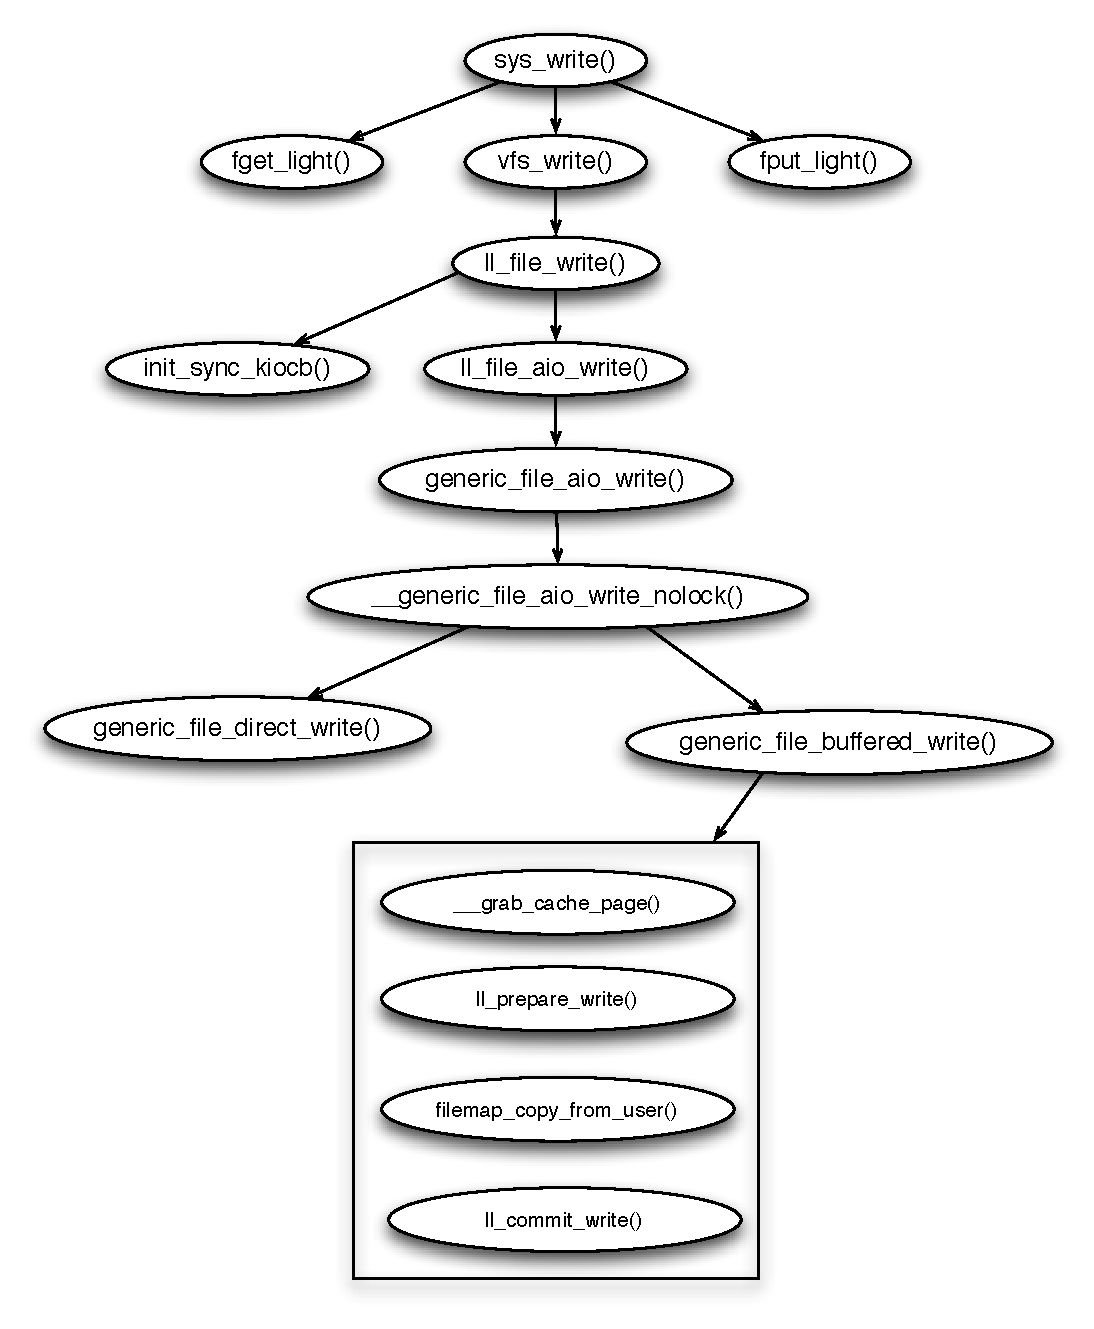
\includegraphics[width=4.5in]{img/lite_write}
\caption{System call graph on the write path as in Linux kernel 2.6.22-14.}
\end{figure}


\subsection{Read-Ahead}

Lustre client read-ahead happens in read-page and is controlled by a
structure, \url{ll_readahead_state}, which is defined in
\url{lustre/llite/llite_internal.h}. This is a per-file structure and encodes
the following information:

\begin{itemize} 

\item \textbf{Read history} (a) how many contiguous reads have happened; (b)
if it is stride read mode, then how many contiguous stride reads have happened;
and (c) stride gap and stride length.

\item \textbf{Read-ahead} windows (i.e., read-ahead window starting and end
points). The more contiguous read happens, the longer the read-ahead window
grows.

\item State information that helps to \textbf{detect read-ahead pattern}.

\end{itemize}

The read-ahead algorithm is described below where each client could read-ahead
a maximum of 40MB:

\begin{enumerate}

\item In read-page (\url{ll_readpage}), the read-ahead state of the file will be
updated according to the current status.
    \begin{enumerate}
     
    \item If this page offset is located in a contiguous window (in +8, -8 window
	with the last page), then \url{ras_consecutive_requests} (defined by
	\url{ll_readahead_state}) will increase by 1. If it is the first page of this
	read, the read-ahead window length will increase by 1MB.  So if the read is
	contiguous, the read-ahead window increases with an increasing number of read
	opeartions.


    \item If this page is not inside the contiguous window, then it will check
    whether it is in stride-read mode. In this case, it will compare current
    stride length/stride gap with past history. If they are equal, then
    \url{ras_consecutive_stride_requests} will be increased by 1. If it is the
    first page of this read, stride read-ahead window will also increase by
    1MB.

    \item If page is neither in contiguous window nor in stride-contiguous
    window, then all the read-ahead state will be reset. For example,
    \url{ras_consecutive_pages} and \url{ras_consecutive_requests} will be
    reset to 0.

    \end{enumerate}

\item Next, read page will do real read-ahead according to the state updated
in the previous step.

     \begin{enumerate}

      \item Increase the read-ahead window and try to cover all the pages for
      this read. This explains why large reads perform better than small
      reads.
       
       \item Adjust the read-ahead window according to the real file length and
       calculate how many pages will be read in this read-ahead.
       
      \item Do actual read-ahead.
    \end{enumerate}

\end{enumerate}

There is a read-ahead stats file in the proc
(\url{/proc/fs/lustre/llite/XXXXX/read_ahead_stats}) where states of read
ahead can be viewed.

